\documentclass{article}

\usepackage[utf8]{inputenc}   %for german letters ä,ö...
\usepackage[ngerman]{babel}   %german settings
\usepackage{amsmath}
\usepackage{amssymb}
\usepackage{tikz}
\usepackage{caption}
\usepackage[left=3cm,right=3cm,top=2cm,bottom=3cm]{geometry}
\usepackage{siunitx}
\usepackage{esdiff}
\usepackage{braket}
\usepackage{booktabs}
\usepackage[outdir=./]{epstopdf}

\sisetup{locale = DE}

\newcommand{\RM}[1]{\MakeUppercase{\romannumeral #1}}

\newcommand{\coord}[2]{%
  
  \draw [->] (#1,#2)--(#1+2,#2);
  \draw [->] (#1,#2)--(#1,2+#2);
  \draw [->] (#1,#2)--(#1-0.8,#2-0.8);
  \draw (#1+0.2,#2+1.9) node {$z$};
  \draw (#1+2.2,#2) node {$y$};
  \draw (#1-0.9,#2-0.9) node {$x$};
}

\usepackage{subcaption}

\usepackage[backend=bibtex8,sorting=none]{biblatex}
\addbibresource{refs.bib}

\begin{document}
\setlength{\parindent}{0em}   %Einrücken verhindern
\title{Physikalisches Praktikum \RM{4}\\Versuch 443\\Kernmagnetische Relaxation}
\author{Friedrich Hübner \qquad s6frhueb@uni-bonn.de \qquad 2897111\\
  Kilian Bönisch \ \ \ \qquad s6kiboen@uni-bonn.de \qquad 2897138}
\date{23.10.17}

\maketitle

\thispagestyle{empty}

\newpage

\section{Einleitung}
In diesem Versuch wird das Verhalten von Spin-$\frac{1}{2}$-Teilchen in einem äußeren Magnetfeld untersucht. Dafür wird eine Probe mit Mineralöl in dem Magnetfeld platziert und die Dynamik des Spins der Protonen beobachtet. Charakteristische Zeitkonstanten die mit der Spin-Spin und Spin-Gitter Wechselwirkung zusammenhängen werden bestimmt.


\section{Theoretische Grundlagen}

\subsection{Spin-$\frac{1}{2}$-Teilchen im konstanten Magnetfeld}
Teilchen mit Spin $\vec{S}$ und gyromagnetischen Verhältnis $\gamma$ haben ein magnetisches Moment
\begin{align*}
  \vec{\mu}=\gamma\vec{S}.
\end{align*}
In einem Magnetfeld $\vec{B}$ ist der Hamiltonoperator (für die Spinwellenfunktion) also gegeben durch
\begin{align}
  H=-\vec{\mu} \cdot \vec{B}=-\gamma \vec{B} \cdot \vec{S} \label{hamilton1}
\end{align}

Für eine anschauliche Beschreibung wird der Bloch-Vektor durch die Erwartungswerte der Pauli-Matrizen definiert:
\begin{align*}
  \vec{K}= \left( \begin{array}{c}
                    \braket{\sigma_x} \\
                    \braket{\sigma_y}\\
                    \braket{\sigma_z}
                  \end{array} \right).
\end{align*}
Aus dem Ehrenfest-Theorem und der Kommutatorrelation für Pauli-Matrizen folgt aus (\ref{hamilton1})
\begin{align}
  \diff{\vec{K}}{t}=\gamma \vec{K} \times \vec{B}.
\end{align}
Die (mittlere) Magnetisierung präzediert also um $\vec{B}.$ \\ \\

Im Folgenden wird die $z$-Achse als Quantisierungsachse gewählt, es soll also $\vec{B}=B\vec{e}_z$ gelten. Für Spin-$\frac{1}{2}$-Teilchen gibt es nur zwei mögliche Eigenwerte $m_z$ von $\vec{S}_z/\hbar$:
\begin{align*}
  m_z=\pm \frac{1}{2}.
\end{align*}
Es handelt sich also wie in Abbildung \ref{aufspaltung} zu sehen um ein zwei-Niveau-System.

\begin{figure}[h]
  \centering
  \begin{tikzpicture}
    \draw (0,0)--(1,0);
    \draw (1,0)--(1.5,1);
    \draw (1,0)--(1.5,-1);
    \draw (1.5,1)--(4,1);
    \draw (1.5,-1)--(4,-1);
    \draw [<->] (2,0.9)--(2,-0.9);
    \draw (3,0) node {$\Delta E=\gamma\hbar B$};
    \draw (4.8,1) node {$m_z=-\frac{1}{2}$};
    \draw (4.8,-1) node {$m_z=\frac{1}{2}$};
  \end{tikzpicture}
  \caption{Aufspaltung des Energieniveaus durch äußeres Magnetfeld}
  \label{aufspaltung}
\end{figure}

Wird nun ein Probe aus $N$ Teilchen in das Magnetfeld gebracht so folgt beim thermischen Gleichgewicht aus der Boltzmann-Verteilung
\begin{align*}
  \frac{N_2}{N_1}=\exp \left( -\frac{\Delta E}{k_\mathrm{B}T} \right),
\end{align*}
wobei $N_1$ ($N_2$) die Besetzungszahl des energetisch niedrigeren (höheren) Zustandes, $k_\mathrm{B}$ die Boltzmann-Konstante und $T$ die Temperatur ist. Die gesamte Magnetisierung in $z$-Richtung ist gegeben durch 
\begin{align*}
  M_z=(N_1-N_2)\mu
\end{align*} 
mit $\mu=\gamma\hbar/2$, im thermischen Gleichgewicht gilt also
\begin{align*}
  M_z=M_0=N\mu\tanh \left(  \frac{\mu B}{k_\mathrm{B}T}\right).
\end{align*}

Bei ausgeschaltetem Magnetfeld ist die Probe zu Beginn unpolarisiert, es gilt also $M_z=0$. Nach \cite{manual} wird der Polarisationsvorgang nach Anschalten des Magnetfeldes durch 
\begin{align*}
  \diff{M_z}{t}=\frac{M_0-M_z}{T_1}
\end{align*}
beschrieben, wobei $T_1$ die materialabhängige longitudinale Relaxationszeit ist. Die Lösung der Differentialgleichung mit der Anfangsbedingung $M_z(0)=0$ ist
\begin{align}
  M_z(t)=M_0\left( 1-e^{-t/T_1} \right).
\end{align}

\subsection{Spin-$\frac{1}{2}$-Teilchen im magnetischen Wechselfeld}
Nun wird die Dynamik des Spins unter Einfluss eines zeitabhängigen magnetischen Feldes untersucht, dazu wird das Feld 
\begin{align*}
  \vec{B}(t)= \left( \begin{array}{c}
                    B_1\cos\omega t\\
                    B_1\sin \omega t \\
                    B_0
                  \end{array} \right)
\end{align*}
betrachtet. Die resultierende Schrödingergleichung
\begin{align}
i\hbar \diff{}{t} \ket{\psi}=H(t)\ket{\psi} \label{hamilton2}
\end{align}
ist nicht mehr trivial lösbar. Um (\ref{hamilton2}) zu vereinfachen wird das Problem in einem mit $\vec{B}$ rotierendem Bezugssystem betrachtet:
\begin{align*}
  \ket{\psi} \rightarrow \ket{\tilde{\psi}}=\exp \left(  i\omega t \vec{S}_z/\hbar\right) \ket{\psi}.
\end{align*}
Für die transformierten Zustände folgt aus (\ref{hamilton2}) die Gleichung
\begin{align*}
  i\hbar \diff{}{t}\ket{\tilde{\psi}}= -\gamma \vec{B}_\mathrm{eff} \cdot \vec{S} \ket{\tilde{\psi}}
\end{align*}
mit dem effektiven Magnetfeld 
\begin{align*}
  \vec{B}_\mathrm{eff}=\left( \begin{array}{c}
                    B_1\\
                    0\\
                    B_0+\omega/\gamma
                  \end{array} \right).
\end{align*}
Im rotierenden Bezugssystem präzidiert die (mittlere) Magnetisierung also um $\vec{B}_\mathrm{eff}$. \\ \\
Für den Fall, dass $B_0=-\omega/\gamma$ gilt, rotiert die Magnetisierung im rotierenden Bezugssystem um die $x$-Achse. Wird das Magnetfeld z.B. für eine Dauer von $t=\pi/(2\gamma B_1)$ eingeschaltet kann eine anfängliche Magnetisierung in $z$-Richtung in die $x$-$y$-Ebene gedreht werden ($\pi/2$-Puls). Der $\pi/2$-Puls ist elementar für den Versuch, da mit dem Aufbau nur die Magnetisierung in der $x$-$y$-Ebene gemessen werden kann. \\ \\
Wird ein $\pi/2$-Puls auf eine in $z$-Richtung polarisierte Probe angewendet wird die Gesamtmagnetisierung in der $x$-$y$-Ebene aufgrund von Wechselwirkungen der Teilchen untereinander exponentiell abfallen (siehe \cite{manual}). Mit der dafür charakteristischen Zeit, der transversale Relaxationszeit $T_2$, gilt also
\begin{align}
  M_{x/y}(t)=M_{x/y}(0) e^{-t/T_2},
\end{align}
dieses abnehmende Signal welches auf dem Oszilloskop sichtbar wird nennt sich FID (free induction decay).

\subsection{Hahn-Spinecho-Sequenz}
In der Praxis ist das Magnetfeld im Bereich der Probe nicht homogen. Das führt nach ??? dazu, dass die effektive transversale Relaxationszeit durch
\begin{align*}
  \frac{1}{T_2^*}=\frac{1}{T_{2,\mathrm{inhom}}}+\frac{1}{T_2}
\end{align*}
gegeben ist, $T_{2,\mathrm{inhom}}$ ist dabei vom Magnetfeld abhängig. \\ \\
Die Hahn-Spinecho-Sequenz erlaubt die Messung von $T_2$. Dazu wird nach einem $\pi/2$-Puls und einer Wartezeit $\tau$ ein $\pi$-Puls auf die Probe gegeben. Nach einer weiteren Wartezeit $\tau$ erreicht die Magnetisierung ein Maximum welches unabhängig von $T_{2,\mathrm{inhom}}$ ist. Das Zustandekommen lässt sich gut an Abbildung \ref{hahn} nachvollziehen. Wenn das Magnetfeld $B_1$ örtlich schwankt präzedieren die Magnetisierungen an verschiedenen Orten etwas langsamer bzw. schneller als das rotierende Bezugssystem. Durch den $\pi$-Puls laufen die Magnetisierungsvektoren anschließend wieder zusammen und sind so an einem Zeitpunkt wieder parallel. 

\begin{figure}[h]
  \centering
  \begin{tikzpicture}
    \coord{0}{0}
    \draw [->,line width=0.5mm](0,0)--(0,1.5);
    \draw [->] (3,1)--(4,1);
    \draw (3.5,1.3) node {$\pi/2$};
    \coord{5}{0}
    \draw [->,line width=0.5mm](5,0)--(6.5,0);
    \draw [->] (8,1)--(9,1);
    \draw (8.5,1.3) node {$\tau$};
    \coord{10}{0}
    \draw [->,line width=0.5mm](10,0)--(11,0.5);
    \draw [->,line width=0.5mm](10,0)--(11.1,-0.6);
    \draw [->] (11.3,0) arc (0:40:0.7);
    \draw [->] (11.3,0) arc (0:-40:0.7);
    \draw [->] (0,-3)--(1,-3);
    \draw (0.5,-2.7) node {$\pi$};
    \coord{2}{-4}
    \draw [->,line width=0.5mm](10-8,0-4)--(9-8,0.5-4);
    \draw [->,line width=0.5mm](10-8,0-4)--(8.9-8,-0.6-4);
    \draw [<-] (0.7,-3.95) arc (180:140:0.7);
    \draw [<-] (0.7,-4.05) arc (180:220:0.7);
    \draw [->] (5,-3)--(6,-3);
    \draw (5.5,-2.7) node {$\tau$};
    \coord{8}{-4}
    \draw [->, line width=0.5mm] (8,-4)--(6.5,-4);
  \end{tikzpicture}
  \caption{Hahn-Spinecho-Sequenz im rotierenden Bezugssystem, die Magnetisierung (fett eingezeichnet) präzediert abhängig vom Magnetfeld schneller bzw. langsamer.}
  \label{hahn}
\end{figure}

\section{Durchführung}
\subsection{Aufbau und Justage}
Der Aufbau besteht aus 

\begin{itemize}
  \item einem Permanentmagneten,
    \item einem PS2-Controller zur Regelung der Magnettemperatur und des Magnetfeldgradienten,
      \item dem Mainframe an dem die Pulssequenzen eingestellt werden und
        \item einem digitalen Oszilloskop.
\end{itemize}

Zunächst wird mit dem PS2 Controller eingestellt, dass die aktuelle Magnettemperatur gehalten wird. Dies ist wichtig, da sich sonst das Megnetfeld bei Temperaturschwankungen ändern kann. \\ \\
Für eine erste Justage wird nun die Pickup-Probe in den Magneten eingesetzt. Diese besteht aus einer einfachen Spule. An dem Mainframe wird als Puls ein Rechteckpuls (Puls A) mit Pulslänge $A_{len}=2,5\mu$s eingestellt. Die Periode (nach welcher Zeit die Pulssequenz sich wiederholt) wird auf $100$ms gestellt. Es muss immer darauf geachtet werden, dass die Periode deutlich größer als die Pulslänge ist. Auf dem Oszilloskop kann nun eine zum Strom der Spule proportionale Spannung beobachtet werden (siehe Abbildung \ref{fig:pickup}). Das Signal hat bereits die erwünschte Form und es sind keine Einstellungen am Magneten notwendig.\\ \\
Nun wird die eigentliche Probe mit Mineralöl in den Magneten eingesetzt. Auf dem Oszilloskop kann nun nach einem $\pi/2$ Puls das FID Signal beobachtet werden. Die Dauer für einen $\pi/2$-Puls wird ermittelt indem die Amplitude des Antwortsignals maximiert wird. Die so ermittelte Pulslänge liegt bei $2,46 \mu$s. Die Frequenz des RF-Pulses und der Magnetfeldgradient werden so eingestellt, dass die Amplitude und die Zerfallszeit des FID Signals maximal werden und keine Nachschwingungen zu erkennen sind. Die ermittelte Resonanzfrequenz liegt bei $21,16272$MHz. Das FID Signal ist in Abbildung \ref{fig:FID} zu sehen. \\ \\
Für eine genauere Bestimmung der Zeit für einen $\pi/2$-Puls wird die Zeit für einen $\pi$-Puls bestimmt indem das Antwortsignal minimiert wird. Die ermittelte Zeit für einen $\pi$-Puls ist $4,92\mu$s, welche genau zu unserer Zeit für den $\pi/2$-Puls passt.

\subsection{Rabi-Oszillationen}
Für Puls A und Pulslängen zwischen $0,5\mu$s und $12\mu$s wird die Magnetisierung in der x-y-Ebene gemessen. Gemessen wird dabei sowohl die Amplitude in der Ebene (Envelope Signal) als auch in einer Raumrichtung der Ebene (In-Phase Signal). Erwartet wird ein oszillierendes Signal in Abhängigkeit der Pulslänge. 

\subsection{Longitudinale Relaxationszeit}
Die Longitudinale Relaxationszeit wird mit zwei verschiedenen Methoden gemessen. \\ \\
Bei der Sättigungs-Zurückgewinnung wird die Probe zunächst einem $\pi/2$-Puls ausgesetzt und anschließend nach einer Wartezeit $\tau$ die Magnetiserung in z-Richtung gemessen (wieder durch einen $\pi/2$-Puls). Durch die Variation von $\tau$ lässt sich die longitudinale Relaxationszeit ermitteln. \\ \\
Bei der Polarisations-Zurückgewinnung unterscheidet sich das Prozedere nur dahingehend, dass die Probe zu Beginn einem $\pi$-Puls ausgesetzt wird. Dadurch wird die Magnetisierung in die negative z-Richtung gedreht. Wieder wird die Amplitude für verschiedene $\tau$ aufgenommen.

\subsection{Homogene Transversale Relaxationszeit}
Die homogene transversale Relaxationszeit wird mit den drei vorgestellten Pulssequenzen ermittelt. Bei der Hahn-Spinecho-Sequenz wird dazu manuell für verschiedene Wartezeiten $\tau$ das Antwortsignal aufgenommen. Bei der Carr-Purcell und der Meiboom-Gill-Sequenz reicht eine Pulssequenz mit $N=20$ Perioden.\\ \\
Um die Carr-Purcell und die Meiboom-Gill-Sequenz vergleichen zu können wird noch die Änderung der Signale bei variierendem Magnetfeldgradienten untersucht.

\begin{figure}[h]
  \centering
  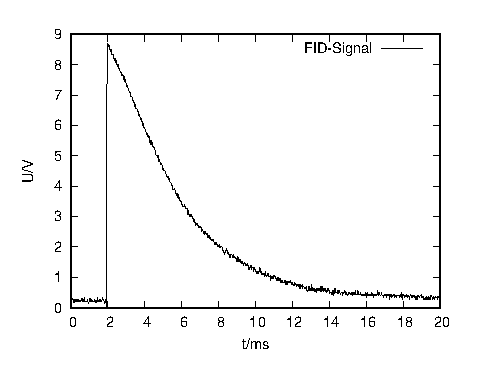
\includegraphics[width=0.75\linewidth]{data/p402_443_data/FID_1/FID_1.eps}
  \caption{FID Signal}
  \label{fig:FID}
\end{figure}


\section{Auswertung}
\subsection{Bestimmung der Lebensdauer}
Für die Bestimmung der Lebensdauer sind zwei Fehler relevant. Zum einen der statistische Fehler durch die Poissonverteilung der Zählwerte und zum anderen die Zahl der Zufallsereignisse. Die Zahl der Zufallsereignisse trägt für jedes der zehn Zählintervalle gleich bei, da keine zeitliche Korrelation besteht. Somit wird bei der Auftragung der Zählereignisse gegen die Zeit die Form

\begin{align}
  N(t)=A e^{-t/\tau}+B
  \label{eq:fit_lebensdauer}
\end{align}
 erwartet. $B$ entsteht dabei durch die Zahl der Zufallsereignisse pro Sichtzähler.
Insgesamt wurden $N_s=2054703$ Startsignale ausgelöst. Da der Teil der Startsignale, der auch zu einer Zählung eines Myonenzerfalls geführt hat, verschwindend gering ist, folgt, dass das Gate für die Messung ungefähr $N_s \cdot \SI{10}{\micro\second}\approx\SI{20.5}{\second}$ geöffnet war. Die Zahl der Zufallsereignisse lässt sich nun durch Multiplikation mit der Rate an Stopsignalen berechnen. Es wurden in der gesamten Zeit von 13 Tagen und 2 Stunden 4314850 Stopsignale ausgelöst. Somit folgt für die Zahl der Zufallsereignisse 
\begin{align*}
  N_z\approx 78.
\end{align*}
Diese Abschätzung kann durch Anpassung der Funktion (\ref{eq:fit_lebensdauer}) mit dem erhaltenen $B$ verglichen werden. Aus der Anpassung folgt
\begin{align*}
  A&=1621 \pm 80\\
  \tau&=\SI[separate-uncertainty = true]{2.2(1)}{\micro\second}\\
  B&=9 \pm 7.
\end{align*}
Da es zehn Sichtzähler gibt gilt im Idealfall $N_z=10B$. Dies stimmt auch grob, allerdings ist der Fehler von $B$ aufgrund der geringen Zählraten fast so groß wie $B$ selbst. Die Lebensdauer von Myonen wurde zu $\tau = \SI[separate-uncertainty = true]{2.2(1)}{\micro\second}$ bestimmt. Die Auftragung der Daten sowie die Anpassungskurve sind in Abbildung \ref{fig:lebensdauer} zu sehen. Die Daten befinden sich in Tabelle \ref{tab:sichtzaehler}.

\begin{figure}[h]
  \centering
  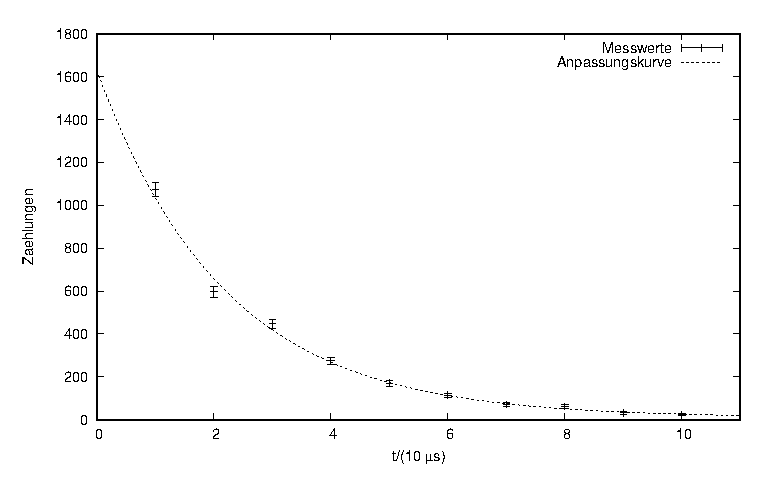
\includegraphics[width=0.8\textwidth]{./data/lebensdauer.eps}
  \caption{Kurve zur Messung der Lebensdauer von Myonen}
  \label{fig:lebensdauer}
\end{figure}


\begin{table}[h]
    \centering
    \caption{abgelesene Zählereignisse von Sichtzählern zur Lebensdauerbestimmung}
    \label{tab:sichtzaehler}
    \begin{tabular}{c | c c c c c c c c c c}
      Sichtzähler &1&2&3&4&5&6&7&8&9&10\\ \hline
      Zählungen &1072&596&447&274&170&114&71&61&32&25\\
    \end{tabular}
  \end{table}

\section{Auswertung}
\subsection{Graphit}
\subsubsection{Grobe Struktur}
\begin{figure}
\centering
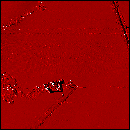
\includegraphics[scale=1]{data/graphit/raw_big.png}
\caption{Grobe Graphitstruktur (Seitenlänge 200nm)}
\label{fig:raw_big}
\end{figure}
In Abb. \ref{fig:raw_big} ist eine Aufnahme mit der Seitenlänge 200nm (CCM-Methode) dargestellt. Man kann eine grobe Struktur unten links, sowie mehrere Kanten erkennen.

\subsubsection{Atomare Auflösung}
Unsere Spitze war geeignet, um atomare Auflösung bei Graphit zu erreichen.
\begin{figure}
\centering
\includegraphics[scale=1]{data/graphit/raw.png}
\caption{Gemessene Graphitstruktur (Seitenlänge 4nm)}
\label{fig:raw}
\end{figure}
\begin{figure}
\centering
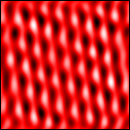
\includegraphics[scale=1]{data/graphit/2nm_edit2.png}
\caption{Graphitstruktur mit Fourierfilter}
\label{fig:edit}
\end{figure}
\begin{figure}
\centering
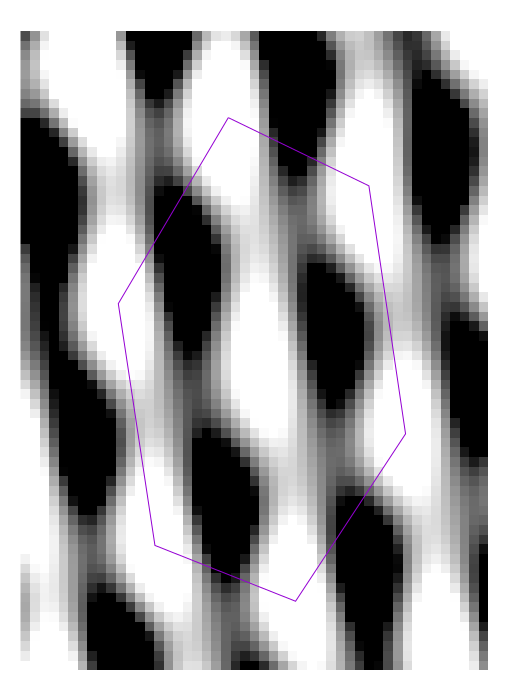
\includegraphics[scale=0.35]{data/graphit/graphit.png}
\caption{Ausschnitt mit ermittelten Mittelpunkten}
\label{fig:small}
\end{figure}
In Abb. \ref{fig:raw} ist das gemessene Bild (CHM-Methode) dargestellt. Da das Bild stark verrauscht ist, wurde ein Fourierfilter angewendet. Das Ergebnis ist in Abb. \ref{fig:edit} dargestellt. Man kann gut das sechseckige Gitter, dass die weißen Bereiche aufspannen, erkennen. Das sind die Punkte, in denen zwei Kohlenstoffatome übereinander liegen. Es handelt sich also nicht um die sechseckige Graphitstruktur, sondern nur um einen Teil davon. Für die Auswertung der Winkel können diese Punkte aber trotzdem verwendet werden, da die Winkel der Gitterstruktur gleich den Winkeln der Sechsecke sind.\\

In einem kleinem Ausschnitt (siehe Abb. \ref{fig:small}) wird nun ein solches Sechseck vermessen. Die Mittelpunkte der weißen Bereiche relativ zum weißem Bereich in der Mitte sind in Tab.\ref{tab:points} dargestellt (Fehler etwa $\Delta x,\Delta y=$ 0,01 nm).

\begin{table}
\centering
\caption{Bestimmte Mittelpunkte der weißen Bereiche}
\begin{tabular}{ccc}
\toprule
n & x/nm & y/nm\\
\midrule
1 & -0,05 &-0,41\\
2 & 0,18&	-0,3\\
3 & 0,24&	0,1\\
4 & 0,06&	0,37\\
5 & -0,17&	0,28\\
6 & -0,23&	-0,11\\
\bottomrule
\end{tabular}
\label{tab:points}
\end{table}
 
Die Punkte bilden offensichtlich kein regelmäßiges Sechseck. Das liegt daran, dass das Bild verzerrt wurde. Um es zu entzerren, drehen wir erst das Bild um den Winkel $\phi$, so dass die Verzerrungsachse in Richtung y-Achse zeigt. Dann verzerren wir das Bild in Richtung y-Achse um den Faktor $\alpha$. Die einzelnen Punkte sollten dann möglichst auf einem Kreis mit Radius $r$ liegen. Dazu sollte der Abstand aller der Punkte zum Ursprung etwa $r$ sein.\\

Um ein möglichst gutes Ergebnis zu erhalten, machen wir einen Fit über die freien Parameter $\phi, \alpha, r$, um die folgende Funktion zu minimieren:
\begin{align*}
f(\phi,\alpha,r) &= \sum\limits_{n = 1}^6 \left(\left|
\begin{pmatrix}
1 & 0\\
0 & \alpha
\end{pmatrix}
\begin{pmatrix}
\cos{\phi} & \sin{\phi}\\
-\sin{\phi} & \cos{\phi}
\end{pmatrix}
\begin{pmatrix}
x_n\\
y_n
\end{pmatrix}
  \right| - r\right)^2
\end{align*}.
Die rechte Matrix dreht das Polygon und die linke verzerrt die y-Achse. Danach wird von der Norm des Vektors $r$ abgezogen und das Quadrat dieser Abweichung aufsummiert. Somit soll sichergestellt werden, dass alle Punkte am Ende näherungsweise auf einem Kreis liegen. Dabei muss beachtet werden, dass das Original in einer Richtung gestaucht wurde. Somit muss $\alpha > 1$ (um die Stauchung rückgängig zu machen) gelten.\\
Der Fit (siehe Tab.\ref{tab:fit}, Abb. \ref{fig:fit1}, Abb. \ref{fig:fit2}) ergab: $\phi = 91,7^\circ \pm 0,9^\circ, \alpha = 1,6 \pm 0,2, r = 0,4\si{\nano\metre} \pm 0,02\si{\nano\metre}$.\\ 

\begin{table}
\centering
\caption{Punkte nach der Entzerrung}
\begin{tabular}{ccc}
\toprule
n & x/nm & y/nm\\
\midrule
1&	-0,40836&	0,101854\\
2&	-0,305142&	-0,281216\\
3& 0,0929292&	-0,399014\\
4&	0,368084&	-0,116354\\
5&	0,284858&	0,265753\\
6&	-0,103218&	0,38307\\
\bottomrule
\end{tabular}
\label{tab:fit}
\end{table}

\begin{figure}
\centering
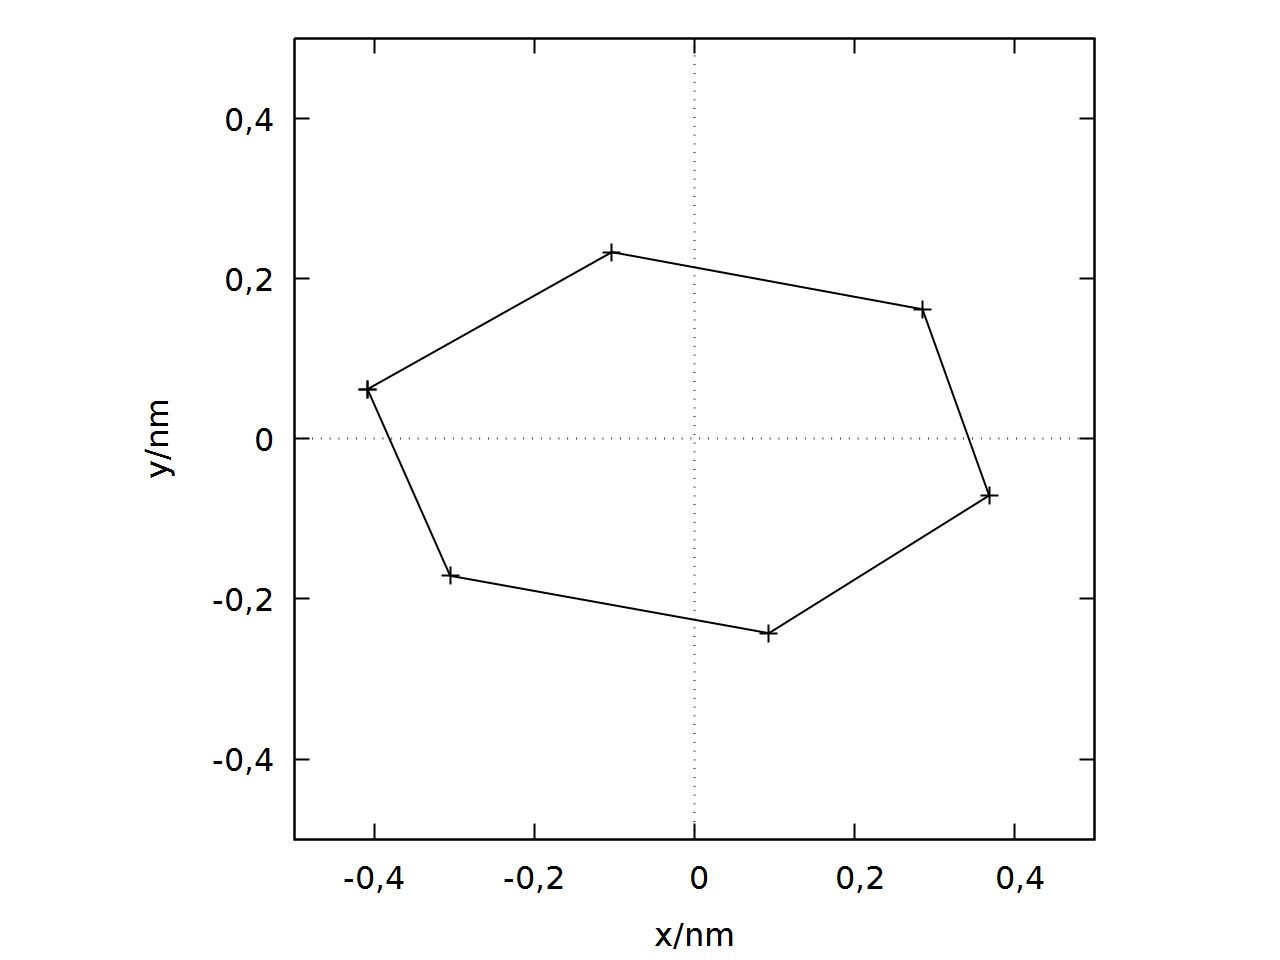
\includegraphics[scale=0.3]{data/graphit/out_rotate_old.png}
\caption{Nach Drehung um Winkel $\phi = 91,7^\circ$}
\label{fig:fit1}
\end{figure}

\begin{figure}
\centering
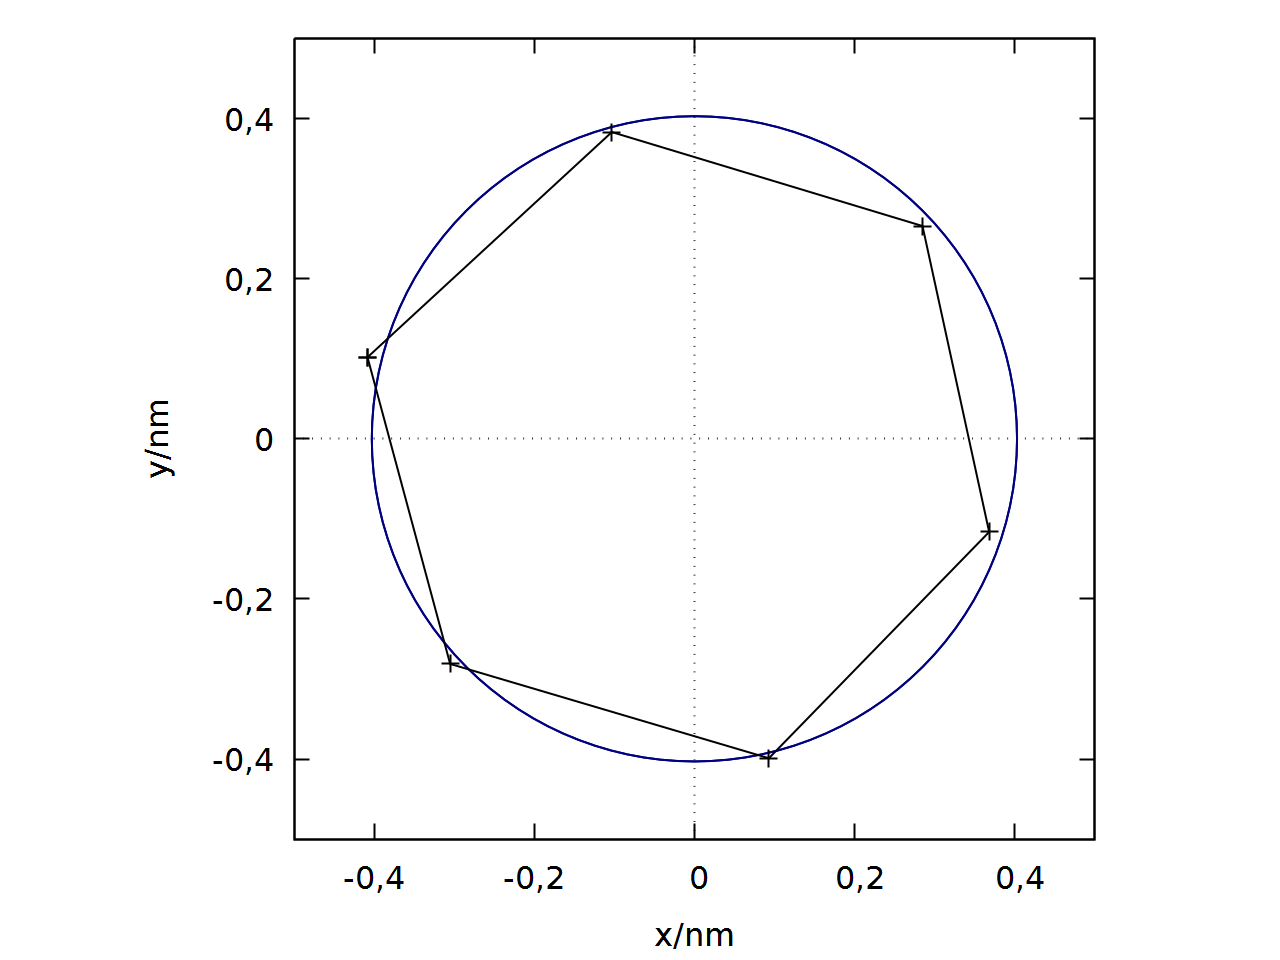
\includegraphics[scale=0.3]{data/graphit/out_rotate.png}
\caption{Nach Drehung und Entzerrung}
\label{fig:fit2}
\end{figure}

Wie man in Abb. \ref{fig:fit2} erkennt, liegen die Punkte jetzt fast auf einem Kreis, sie sind nur etwas verschoben. In Tab. \ref{tab:res} sind die gemessenen Kantenlängen und Innenwinkel aufgetragen. Durch Mittelung (Fehler über Standartabweichung) ergibt sich $l = 0,40 \pm 0,01$ und $\phi = 120^\circ \pm 2,3^\circ$. Dass der Wert für $\phi = 120^\circ$ beträgt, liegt nicht an einer genauen Messung, sondern daran, dass jedes Sechseck eine Innenwinkelsumme von $720^\circ$ hat. Demzufolge ist nur der Fehler ausschlaggebend. Bei $\Delta\phi=2,3^\circ$ kann man davon ausgehen, dass es sich um gleichseitige Sechsecke handelt und somit Graphit eine Gitterstruktur aus regelmäßigen Sechsecken hat.\\

\begin{table}
\centering
\caption{Punkte nach der Entzerrung}
\begin{tabular}{>{$}c<{$}cc}
\toprule
n & l/nm & $\phi/^\circ$\\
\midrule
1 \to 2 & 0,397 & 117,583\\
2 \to 3 & 0,415 & 121,565\\
3 \to 4 & 0,394 & 117,745\\
4 \to 5 & 0,391 & 123,483\\
5 \to 6 & 0,405 & 119,108\\
6 \to 1 & 0,415 & 120,516\\
\bottomrule
\end{tabular}
\label{tab:res}
\end{table}

Um die Atomabstände $a$ von Graphit zu bestimmen, muss beachtet werden, dass die weißen Punkte nur die Atome darstellen, die direkt über einem anderem sind. Drei benachbarte Atome in einem Sechseck bilden ein gleichschenkliges Dreieck mit der Basis $l$ und den Atomabständen $a$ als Schenkel (siehe Abb. \ref{fig:triangle}). Der Winkel an der Spitze beträgt $120^\circ$. Damit ergibt sich
\begin{align*}
a\cdot\sin{\frac{120^\circ}{2}} &= \frac{l}{2}\\
a &= \frac{l}{\sqrt{3}}\\
  &= 0,231 \pm 0,006
\end{align*}. Der Abstand der Atome beträgt also $a = 0,231\si{\nano\metre} \pm 0,006\si{\nano\metre}$.

\begin{figure}
\centering
\definecolor{qqwuqq}{rgb}{0.,0.39215686274509803,0.}
\definecolor{ffffff}{rgb}{1.,1.,1.}
\begin{tikzpicture}[line cap=round,line join=round,>=triangle 45,x=3.0cm,y=3.0cm]
\clip(-1.798235627638573,-1.1694768704984821) rectangle (2.968878775383718,1.243097549118033);
\draw [shift={(0.,0.)},color=qqwuqq,fill=qqwuqq,fill opacity=0.10000000149011612] (0,0) -- (-60.:0.12435950616579888) arc (-60.:0.:0.12435950616579888) -- cycle;
\draw (-0.5,0.8660254037844388)-- (0.5,0.8660254037844386);
\draw (0.5,0.8660254037844386)-- (1.,0.);
\draw (1.,0.)-- (0.5,-0.866025403784439);
\draw (0.5,-0.866025403784439)-- (-0.5,-0.8660254037844384);
\draw (-0.5,-0.8660254037844384)-- (-1.,0.);
\draw (-1.,0.)-- (-0.5,0.8660254037844388);
\draw [dash pattern=on 1pt off 1pt] (0.5,0.8660254037844386)-- (1.5,0.866025403784439);
\draw [dash pattern=on 1pt off 1pt] (0.5,0.8660254037844386)-- (0.,0.);
\draw [dash pattern=on 1pt off 1pt] (0.,0.)-- (0.5,-0.866025403784439);
\draw [dash pattern=on 1pt off 1pt] (0.5,-0.866025403784439)-- (1.5,-0.8660254037844395);
\draw [dash pattern=on 1pt off 1pt] (1.5,-0.8660254037844395)-- (2.,0.);
\draw [dash pattern=on 1pt off 1pt] (1.5,0.866025403784439)-- (2.,0.);
\draw [dotted] (0.5,0.8660254037844385)-- (0.5,-0.8660254037844392);
\draw [dotted] (0.,0.)-- (0.5,0.);
\begin{scriptsize}
\draw [fill=ffffff] (0.,0.) circle (2.5pt);
\draw[color=black] (0.2039524216307892,0.5031584874315245) node {a};
\draw[color=black] (0.2039524216307892,-0.4295378088119736) node {a};
\draw [fill=ffffff] (0.5,0.8660254037844385) circle (2.5pt);
\draw[color=ffffff] (0.5272871376618663,0.9425620758840169) node {$E$};
\draw [fill=ffffff] (0.5,-0.8660254037844392) circle (2.5pt);
\draw[color=ffffff] (0.5272871376618663,-0.790180376692793) node {$F$};
\draw [fill=ffffff] (-1.,0.) circle (2.5pt);
\draw[color=ffffff] (-0.9691722531999137,0.07619084959561201) node {$G$};
\draw [fill=ffffff] (2.,0.) circle (2.5pt);
\draw[color=ffffff] (2.02789184539584,0.07619084959561201) node {$H$};
\draw[color=black] (0.5314324545340595,-0.031587389081414445) node {l};
\draw [fill=ffffff] (1.,0.) circle (2.5pt);
\draw[color=ffffff] (1.041306429813835,0.07619084959561201) node {$F'$};
\draw[color=qqwuqq] (0.08788354920937688,-0.019151438464834462) node {60\textrm{\degre}};
\end{scriptsize}
\end{tikzpicture}
\caption{Zwei Sechsecke in unterschiedlichen Ebenen}
\label{fig:triangle}
\end{figure}


\subsection{Gold}
\begin{figure}
\centering
\includegraphics[scale=1]{data/gold/raw.png}
\caption{Grobe Goldstruktur (Seitenlänge 100nm)}
\label{fig:gold}
\end{figure}
In Abb. \ref{fig:gold} ist eine Aufnahme mit der Seitenlänge 100nm (CCM-Methode) dargestellt.  Da der linke Teil deutlich heller ist, ist er höher als der rechte. Wir denken also, dass die Aufnahme an einer Kante entstanden ist. Im Vergleich zu Graphit wirkt die Aufnahme verschwommen und es bilden sich wolkenartige Strukturen. Dies liegt daran, dass die Ladungsdichte in Gold deutlich homogener verteilt ist als in Graphit. Demzufolge war es uns auch nicht möglich eine Aufnahme mit atomarer Auflösung herzustellen. Um die atomare Oberfläche von Gold zu betrachten, bräuchte man eine andere Methode, wie z.B. ein Rasterkraftmikroskop.

\subsection{TaS$_2$}
\begin{figure}
\centering
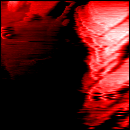
\includegraphics[scale=1]{data/tas2/tas2.png}
\caption{Grobe TaS$_2$-Struktur (Seitenlänge 84,7nm)}
\label{fig:tas2}
\end{figure}
In Abb. \ref{fig:tas2} ist eine Aufnahme mit der Seitenlänge 84,7nm (CCM-Methode) dargestellt. Auch hier kann man grobe Strukturen erkennen, die höher liegen als andere. Eine Abbildung mit atomarer Auflösung aufzunehmen war leider nicht möglich. Demzufolge konnten wir auch keine Ladungsdichtewellen erkennen. 

\newpage
\printbibliography

\end{document}
